\documentclass[12pt,twoside]{article}
\usepackage[dvipsnames]{xcolor}
\usepackage{tikz,graphicx,amsmath,amsfonts,amscd,amssymb,bm,cite,epsfig,epsf,url}
\usepackage[hang,flushmargin]{footmisc}
\usepackage[colorlinks=true,urlcolor=blue,citecolor=blue]{hyperref}
\usepackage{amsthm,multirow,wasysym,appendix}
\usepackage{array,subcaption} 
% \usepackage[small,bf]{caption}
\usepackage{bbm}
\usepackage{pgfplots}
\usetikzlibrary{spy}
\usepgfplotslibrary{external}
\usepgfplotslibrary{fillbetween}
\usetikzlibrary{arrows,automata}
\usepackage{thmtools}
\usepackage{blkarray} 
\usepackage{textcomp}
\usepackage[left=0.8in,right=1.0in,top=1.0in,bottom=1.0in]{geometry}
\usepackage{pifont}
\newcommand{\tick}{\ding{51}}%
\newcommand{\xmark}{\ding{55}}
\input{macros}

\newcommand{\ru}{\rnd{ u}  }
\newcommand{\rd}{\rnd{ d}  }
%\newcommand{\rs}{\rnd{ s}  }
\newcommand{\ri}{\rnd{ i}  }
\newcommand{\re}{\rnd{ e}  }
\newcommand{\rQ}{\rnd{ q}  }
\newcommand{\rC}{\rnd{ c}  }


\begin{document}

\begin{center}
{\large{\textbf{Homework 6}} } \vspace{0.2cm}\\
Due November 5 at 11 pm
\\
\end{center}
\input{hwstatement.tex}\\

\begin{enumerate}

\item (Spam detector) In order to build a spam classifier, we gather the following data. Each row is an email. The first column indicates whether it is spam or not. The remaining columns indicate whether it contains (\tick) or not (\xmark) the word on top.
\begin{center}
{\footnotesize
\begin{tabular}{ |c|c|c|c|c| } 
 \hline
 & Miracle  & Alternative & Medicine & Basketball \\
\hline 
Spam &  \tick  & \tick& \tick & \tick  \\
\hline
Not spam &  \xmark  & \xmark& \tick & \tick  \\
\hline 
Spam &  \tick  & \xmark& \xmark & \xmark  \\
\hline
Not spam &  \xmark  & \tick& \xmark & \xmark  \\
\hline
Spam &  \tick  & \xmark& \xmark & \xmark  \\
\hline
Not spam &  \xmark  & \tick& \xmark & \tick  \\
\hline 
Spam &  \tick  & \xmark& \xmark & \xmark  \\
\hline
Spam &  \xmark  & \tick& \tick & \xmark  \\
\hline
Not spam &  \tick  & \tick& \xmark & \tick  \\
\hline
Not spam &  \xmark  & \xmark& \tick & \tick  \\
\hline 
\end{tabular}
}
\end{center}
We use a Bernoulli random variable $\ry$ to model whether the email is spam ($\ry=1$) or not ($\ry=0$), and a four-dimensional random vector $\rx$ to indicate whether the $i$th word is  ($\rx[i]=1$) or not ($\rx[i]=0$) in the email for $i \in \keys{1,2,3,4}$.
\begin{enumerate}
\item  Your friend recommends that you estimate the conditional pmf of $\ry$ given $\rx$ and then maximize it to produce your estimate. What is the problem with this approach?
\item Apply naive Bayes to classify an email that reads \emph{I hurt my foot playing basketball. %It's a miracle I didn't break it. 
Can you get me some medicine?} 
\item Apply naive Bayes to classify an email that reads \emph{This alternative medicine is amazing, send us all your money!} Explain what shortcoming of the naive Bayes classifier is illustrated by this example.
\end{enumerate}

\item (The Markov property) Let $\ra_1$, $\ra_2$, \ldots, $\ra_n$ be a Markov chain, where for any $1 < i < n$, $\ra_{i+1}$ is conditionally independent of $\ra_1 ,\ldots,\ra_{i-1}$ given $\ra_{i}$, i.e.
\begin{align}
\label{eq:markov_cond_pmf}
p_{ \ra_{ i+1} \cnd \ra_1 ,\ldots,\ra_{i}  }\brac{ a_{i+1} \cnd a_1, a_2, \ldots, a_i } =  p_{ \ra_{i+1}  \cnd \ra_i  }\brac{ a_{ i+1} \cnd a_{i} },
\end{align}
for any values of $a_1$, $a_2$, \ldots, $a_n$. Show that this implies that the future is conditionally independent from the past given the present:
\begin{align}
p_{ \ra_{ i+1},\ra_{i-1} \cnd \ra_i }\brac{ a_{i+1},a_{i-1} \cnd  a_i } = p_{ \ra_{ i+1} \cnd \ra_i }\brac{ a_{i+1} \cnd  a_i } p_{ \ra_{i-1} \cnd \ra_i }\brac{ a_{i-1} \cnd  a_i },
\end{align}
for any $2 \leq i \leq n-1$ and any values of $a_{i-1}$, $a_i$, $a_{i+1}$. (Hint: First show that $p_{ \ra_{ i+1} \cnd \ra_{i-1} , \ra_i}\brac{ a_{i+1}\cnd a_{i-1}, a_{i}  }  = p_{ \ra_{ i+1} \cnd  \ra_i}\brac{ a_{i+1}\cnd a_{i}  } $ for $a_{i-1}$, $a_i$, $a_{i+1}$.)

\item (Mobile phones)
A company that makes mobile phones wants to model the sales of a new model they have just released. At the moment 90\% of the phones are in stock, 10\% have been sold locally and none have been exported. Based on past data, the company determines that each day a phone is sold with probability 0.2 and exported with probability 0.1. We define the following time-homogeneous Markov chain with three states to model this:

\begin{center}
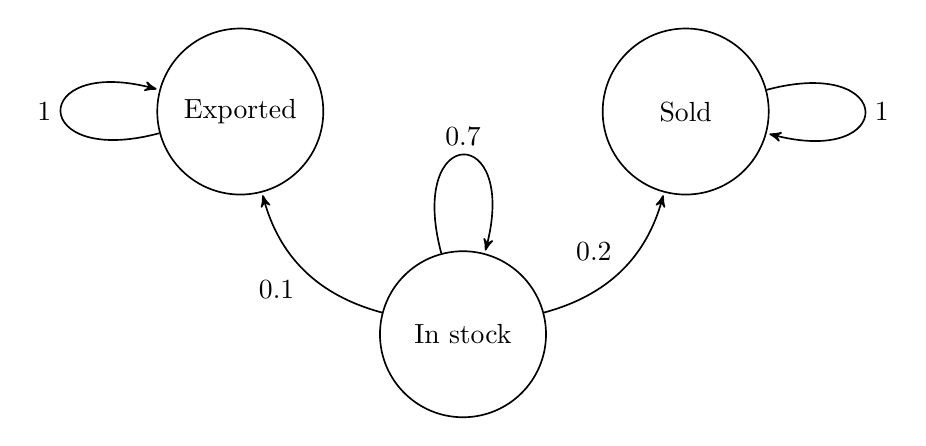
\begin{tikzpicture}[->,>=stealth',shorten >=1pt,auto,node distance=4cm,
                    semithick]
  \tikzstyle{every state}=[text=black]

 \node[state,minimum size = 60pt] (S)                    {In stock};
  \node[state,minimum size = 60pt]         (C) [above right of=S] {Sold};
  \node[state,minimum size = 60pt]         (G) [above left of=S] {Exported};
 
  \path (S) edge    [bend right]      node {0.2} (C)
            edge     [bend left]         node {0.1} (G)
            edge [loop above] node {0.7} (S)
        (C) edge [loop right] node  {1} (C)
        (G) edge [loop left] node  {1} (G);
\end{tikzpicture}
\end{center} 

\begin{enumerate}
\item What is the limit of the state vector $\pi_{i}$ as $i \rightarrow \infty$?
\item Simulate the Markov chain and plot the evolution of the state vector. 
\end{enumerate}

\item (Smoothing) In the application of naive Bayes, instead of computing the conditional pmf $p_{\rnd{x}[i] \cnd \rnd{y}}(x[i]|y)$ empirically, we usually compute the conditional pmf as follows:

$$p_{\rnd{x}[i] \cnd \rnd{y}}(\rnd{x}[i] \cnd y) = \frac{\text{number of samples with label } y \text{ and having feature } x[i] + m}{\text{number of samples with label } y + md},$$

where $m$ is a smoothing constant, and $d$ is the number of features.

\begin{enumerate}
 \item What is the problem with naive Bayes when there is no smoothing ($m=0$) and how does smoothing alleviate this?
  \item Complete the notebook \textit{spam.ipynb}. Which $m$ results in the highest accuracy on the test set? 
  \item In the code, we compare the joint pmf $p_{\rnd{y}, \rnd{x}[1], \cdots, \rnd{x}[d]}(y, \rnd{x}[1], \cdots \rnd{x}[d])$ for $y\in \{0,1\}$. Why is this equivalent to Equation (4.146) in the notes? Why do we need to apply the logarithm in practice?
\end{enumerate}


\end{enumerate}
\end{document}
